\chapter{Figuras}
\label{cap:anexo-figuras}

Este anexo recoge material gráfico complementario a la memoria. Las figuras que acompañan directamente al hilo argumental se mantienen en los capítulos correspondientes; aquí se incluyen aquellas que, por su naturaleza de artefacto autocontenido, se consultan mejor de forma independiente.

\section{Carteles de difusión de las encuestas}
\label{sec:anexo-carteles}

Durante la fase de captación de participantes para las dos encuestas se diseñaron carteles de difusión. Cada cartel resume el objetivo de la encuesta, el tiempo estimado de participación y el enlace de acceso, acompañado de un código QR que redirige al formulario web. El diseño sigue la identidad visual de Dixi, con la mascota como elemento reconocible y la paleta cromática descrita en el capítulo de la aplicación móvil.

\begin{figure}[ht]
    \centering
    % TODO: sustituir el placeholder por la imagen del cartel de difusión de la
    % encuesta de golden standard. Debe mostrar el cartel completo a buena
    % resolución, con el título, la llamada a participar, el tiempo estimado,
    % el código QR y el enlace.
    % 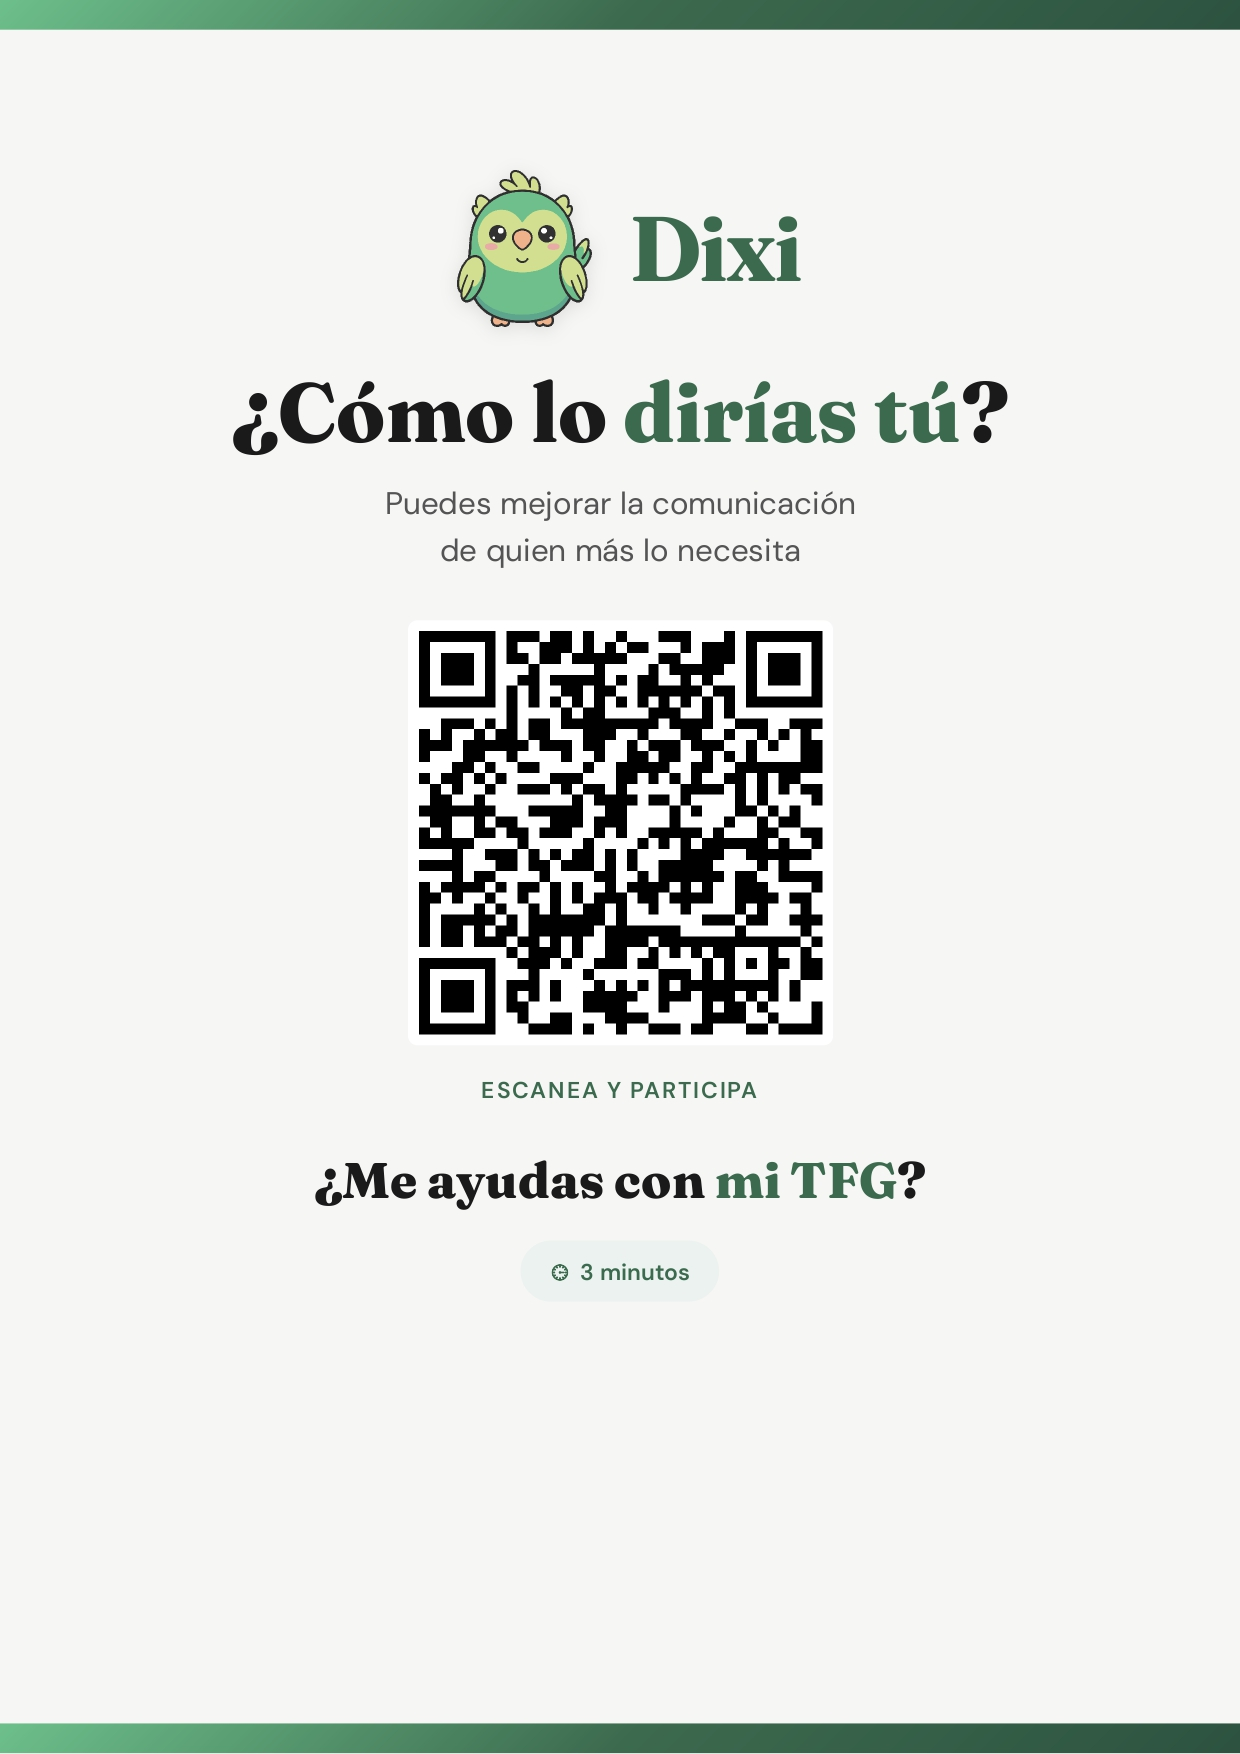
\includegraphics[width=0.7\textwidth]{figures/anexo/cartel-golden.png}
    \placeholderfigura[0.7\textwidth]{8cm}
    \caption{Cartel de difusión de la encuesta de \textit{golden standard}. Se utilizó para captar participantes en los canales personales del autor durante el periodo de recogida de referencias humanas.}
    \label{fig:cartel-golden}
\end{figure}

\begin{figure}[ht]
    \centering
    % TODO: sustituir el placeholder por la imagen del cartel de difusión de la
    % encuesta de naturalidad. Debe mostrar el cartel completo a buena
    % resolución, con el título, la llamada a participar, el tiempo estimado,
    % el código QR y el enlace. Si se usó el mismo cartel para ambas encuestas,
    % eliminar esta figura y actualizar la redacción en la
    % Sección~\ref{sec:anexo-carteles}.
    % 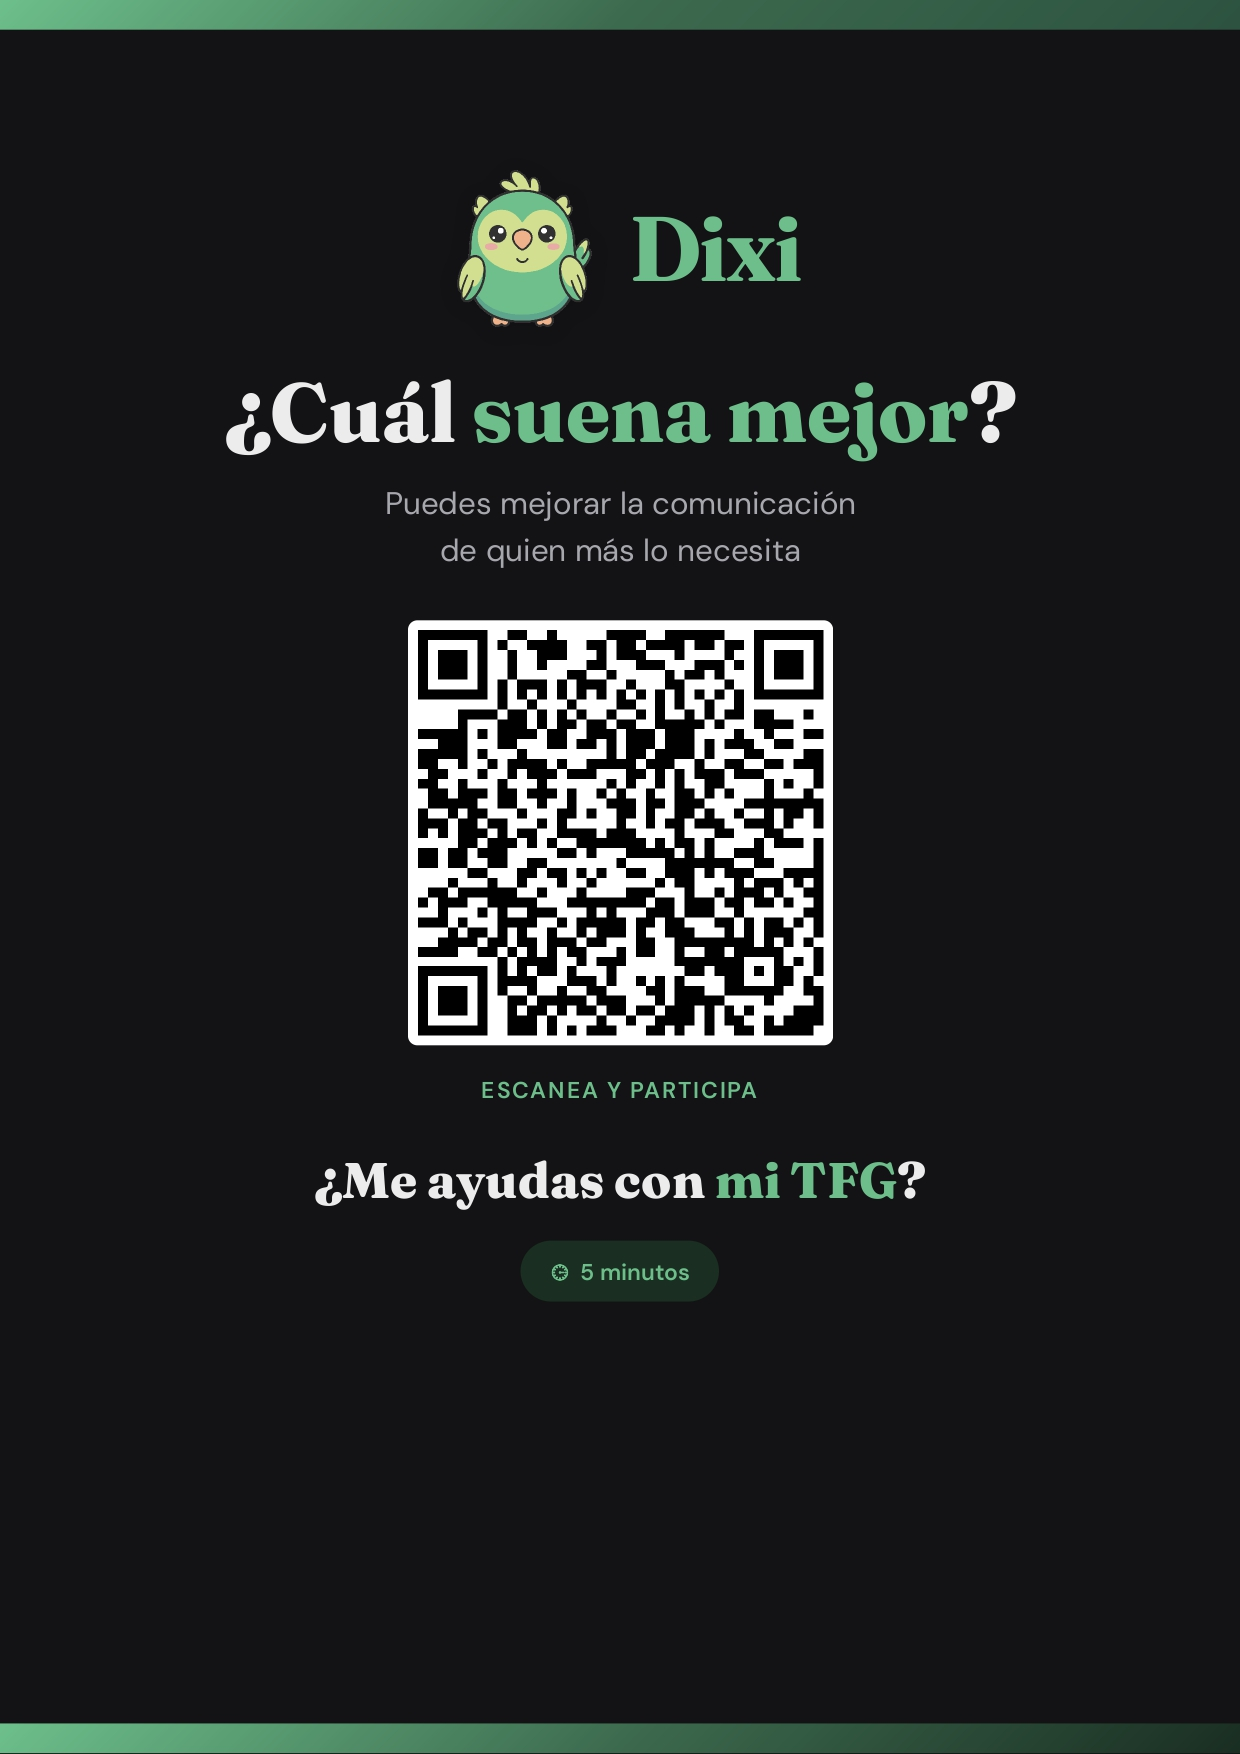
\includegraphics[width=0.7\textwidth]{figures/anexo/cartel-naturalidad.png}
    \placeholderfigura[0.7\textwidth]{8cm}
    \caption{Cartel de difusión de la encuesta de naturalidad. Se utilizó en la convocatoria del estudio de elección forzada entre las tres técnicas base.}
    \label{fig:cartel-naturalidad}
\end{figure}

\section{Interfaces de las encuestas}
\label{sec:anexo-interfaces-encuestas}

Las dos encuestas se desplegaron como aplicaciones web específicas para el proyecto. Las capturas siguientes muestran la pantalla con la que se encontraban los participantes en cada una: la encuesta de \textit{golden standard}, con un campo libre para escribir la frase propia, y la de naturalidad, con la selección de elección forzada entre las frases generadas por las tres técnicas base.

\begin{figure}[ht]
    \centering
    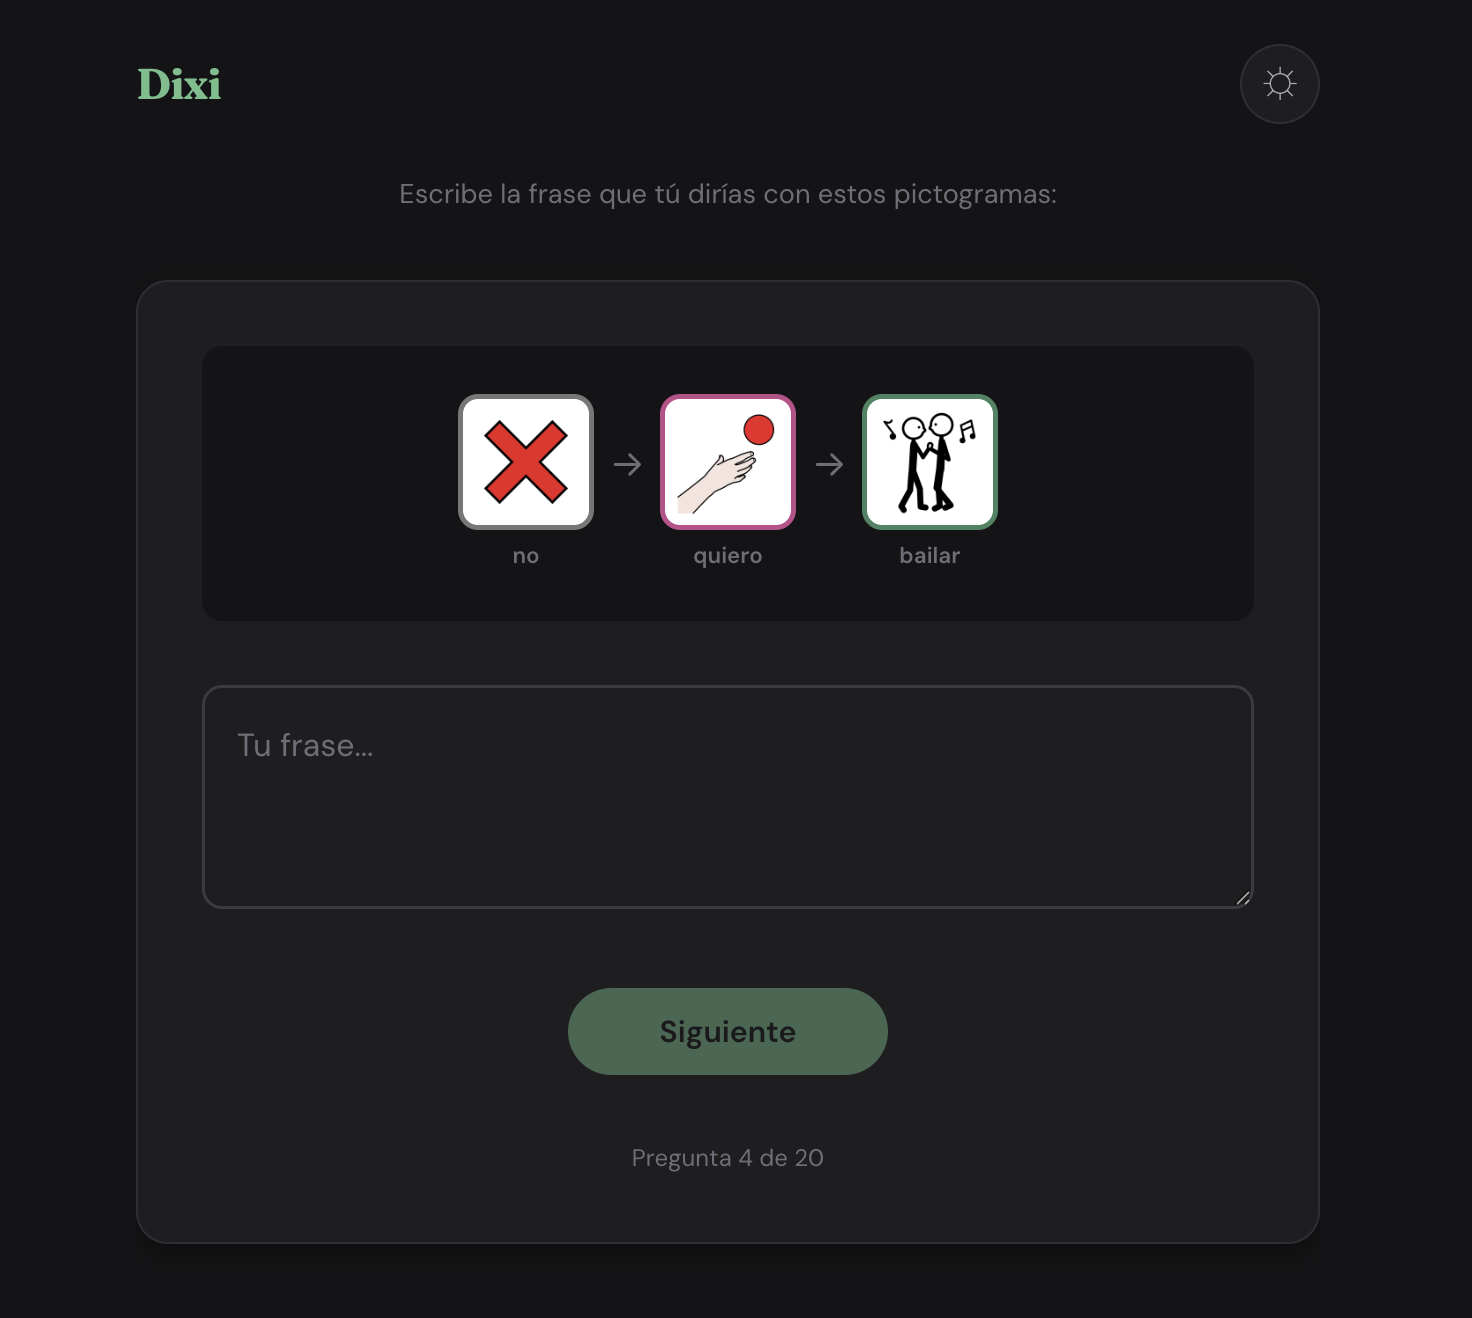
\includegraphics[width=0.7\textwidth]{figures/eval-golden-encuesta.png}
    \caption{Interfaz de la encuesta de \textit{golden standard}. El participante ve la secuencia de pictogramas con sus etiquetas y dispone de un campo libre para escribir la frase que diría.}
    \label{fig:eval-golden-encuesta}
\end{figure}

\begin{figure}[ht]
    \centering
    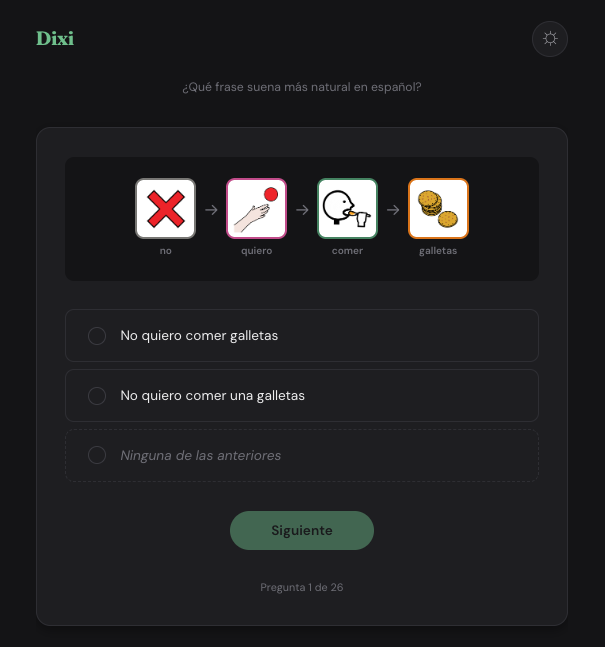
\includegraphics[width=0.7\textwidth]{figures/eval-naturalidad-encuesta.png}
    \caption{Interfaz de la encuesta de naturalidad. El evaluador ve la secuencia de pictogramas junto con las frases generadas por las tres técnicas base, en orden aleatorizado y sin decodificar, y escoge la que le resulta más natural o la opción ``Ninguna de las anteriores''.}
    \label{fig:eval-naturalidad-encuesta}
\end{figure}
